% =====================================================
\chapter{Preliminary Experiments and Baseline Evaluation}
\label{chap:foundations_existing}

This chapter covers two preparatory stages of the research.
The first is a series of foundational experiments --- Vision Transformer, U-Net, DDPM, and classifier-guided conditional diffusion --- carried out to build an intuitive understanding of the key components that drive diffusion-based generative models.
The intent was not to reproduce benchmark-level results but to practically observe how different architectures behave once trained: how the loss evolves, how reconstruction emerges from noise, and how conditioning mechanisms influence the generation process.
The second stage is a systematic evaluation of three state-of-the-art style-transfer frameworks (StyleShot, CSGO, and InstantStyle) against a curated dataset of extreme-weather reference imagery.
This evaluation establishes the performance ceiling of off-the-shelf methods and identifies the precise failure mode --- physically incoherent atmospheric rendering --- that the proposed system in Chapter~\ref{chap:adaptive_proposed} was designed to address.

% =====================================================
\section{Foundational Experiments}
\label{sec:foundations}

\noindent Before engaging with any existing framework, time was spent implementing and observing the underlying building blocks from scratch.
Each experiment captures one essential property of diffusion systems: ViT illustrates the power of attention in capturing global context; U-Net demonstrates how spatial structure is preserved through skip connections; DDPM visualizes the transformation from noise to structure; and classifier-guided diffusion introduces controllability through explicit gradient-based conditioning.
Together, they form the conceptual and empirical foundation upon which later adaptive and style-aware diffusion experiments are built.

% -------------------------------------------------------
\subsection{Vision Transformer (ViT)}
\label{sec:vit}

\noindent The Vision Transformer (ViT)~\cite{dosovitskiy2020vit} experiment was designed to understand how transformer-based vision models capture global relationships in images compared to convolutional architectures.
A compact ViT with a shallow DETR-style~\cite{carion2020endtoendobjectdetectiontransformers} head was implemented to explore how patch embeddings interact with query-based decoding.
Training was performed on CIFAR-10, with images resized to $224\times224$ to fit the patch embedding scheme.
The setup used the Adam optimiser ($3\times10^{-4}$), batch size 64, and 50 epochs of training with ReLU activation and 0.1 dropout.
The network used a 768-dimensional embedding space, 12 attention heads, and a patch size of 16.

DETR (Detection Transformer)~\cite{carion2020endtoendobjectdetectiontransformers} was originally introduced to remove handcrafted detection stages such as anchor boxes or non-maximum suppression, relying solely on attention to perform end-to-end object detection.
It formulates detection as a direct set prediction task using the Hungarian loss for optimal bipartite matching between predicted and ground-truth objects.
In this experiment, while detection itself was not the goal, integrating the DETR-style decoder provided a practical view of how attention can align semantically meaningful tokens, thereby learning structure without explicit convolution.

\paragraph{Results}
The ViT achieved around \textbf{85\% test accuracy} on CIFAR-10.
Attention visualisations clearly revealed that transformer heads concentrated on key object parts (e.g., airplane wings or vehicle bodies) while ignoring background clutter.
Training was smooth, with stable convergence by the 40th epoch.
The experiment reinforced the interpretability and global reasoning capacity of attention, thereby forming the mental framework used later to understand cross-attention in diffusion models.

\begin{figure}[!h]
    \centering
    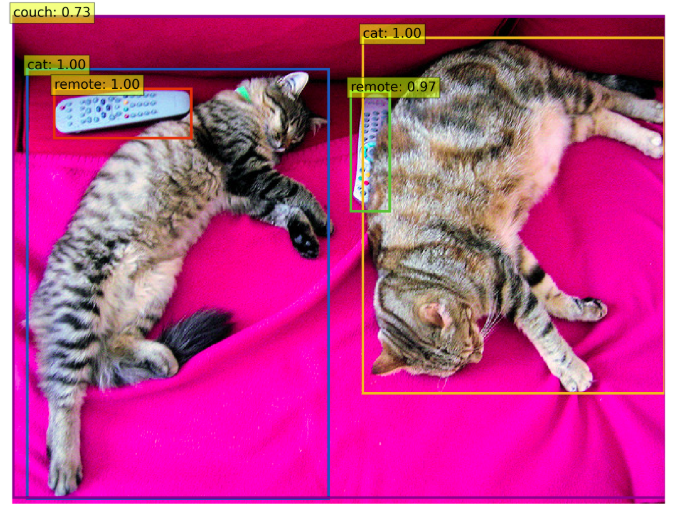
\includegraphics[width=0.65\linewidth]{images/vit_results.png}
    \caption{Vision Transformer on CIFAR-10: attention heads highlighting key semantic regions.}
    \label{fig:vit_results}
\end{figure}

% -------------------------------------------------------
\subsection{U-Net Backbone}
\label{sec:unet}

\noindent The U-Net~\cite{ronneberger2015unet} backbone was explored to understand how skip connections preserve fine structure during reconstruction --- a feature that makes it the default denoising network in diffusion models.
A basic U-Net autoencoder was trained on the Oxford-IIIT Pet dataset ($128\times128$ resolution) for segmentation using Adam ($1\times10^{-3}$), cross-entropy loss, and batch size 8.
Each encoder block contained two $3\times3$ convolutions with ReLU followed by max pooling; the decoder mirrored this with transposed convolutions and symmetric skip connections.
The architecture was intentionally kept simple to focus on reconstruction behaviour rather than architectural sophistication.

\paragraph{Results}
Training converged quickly, with the model accurately recovering spatial boundaries after just a few epochs.
Figure~\ref{fig:unet_segmentation_results} shows clean, sharp segmentation outputs that closely match ground-truth masks.
Skip connections clearly restored high-frequency information lost during downsampling, which explains why the same structure works so effectively in denoising networks.
In diffusion settings, these skip pathways combine with sinusoidal time-step embeddings, giving the model temporal awareness of which stage of denoising it is in and making U-Net both spatially and temporally adaptive.

\begin{figure}[!h]
    \centering
    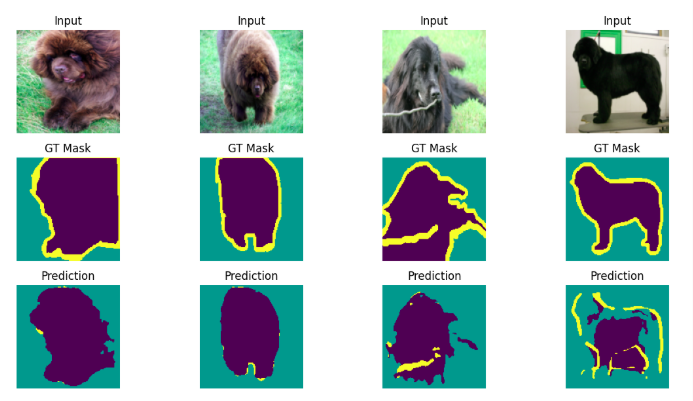
\includegraphics[width=0.55\linewidth]{images/unet_segmentation_results.png}
    \caption{U-Net on Oxford-IIIT Pet: input, ground truth, and reconstructed output.}
    \label{fig:unet_segmentation_results}
\end{figure}

% -------------------------------------------------------
\subsection{Denoising Diffusion Probabilistic Model (DDPM)}
\label{sec:ddpm}

\noindent The DDPM~\cite{ho2020ddpm} experiment visualised the \emph{order from noise} process central to diffusion-based generation.
A U-Net backbone was employed, augmented with sinusoidal time embeddings to encode temporal information.
Training was performed on MNIST (resized to $32\times32$) for 15 epochs using the Adam optimiser ($1\times10^{-4}$) and a linear $\beta_t$ schedule ranging from $1\times10^{-4}$ to $2\times10^{-2}$ over 1000 diffusion steps.
The network learned to predict the clean image $x_0$ from a noisy latent $x_t$ by minimising mean-squared error between the predicted and actual noise.

\paragraph{Results.}
Figure~\ref{fig:ddpm_samples} illustrates the progressive refinement of generated digits.
At the earliest diffusion steps, outputs resemble pure Gaussian noise with no discernible structure.
As sampling proceeds, faint digit contours appear --- a reflection of the model beginning to estimate global shape information.
Midway through the denoising trajectory, the model stabilises coarse structure (loops of 0, stalks of 1 or 9), while fine pixel-level details remain stochastic.
In the final few steps, residual noise is systematically removed, revealing sharply formed digits with clear boundaries and correct topology.

This progression provides an intuitive visualisation of how diffusion models learn to reverse entropy: rather than generating pixels directly, the model gradually transforms a noise distribution into structured data through a sequence of learned conditional transitions.
The experiment also highlights the smooth and interpretable nature of diffusion learning --- unlike GANs~\cite{goodfellow2014gan}, where generation can be abrupt or unstable, diffusion exhibits continuous improvement across time steps, offering clear insight into how the model internalises spatial and probabilistic cues from the dataset.
Despite being trained on a simple dataset, the experiment effectively demonstrates the fundamental mechanics of diffusion, validating the theoretical framework that underpins more advanced models such as Stable Diffusion and InstantStyle.

\begin{figure}[!h]
    \centering
    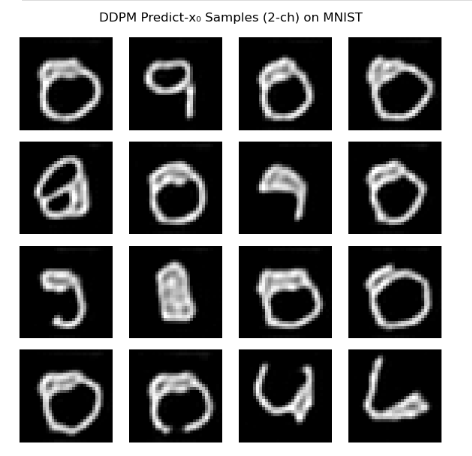
\includegraphics[width=0.65\linewidth]{images/ddpm_samples.png}
    \caption{DDPM on MNIST: progressive denoising from pure noise to clear digits.}
    \label{fig:ddpm_samples}
\end{figure}

% -------------------------------------------------------
\subsection{Conditional Diffusion (Classifier-Guided)}
\label{sec:conditional_diffusion_exp}

\noindent The classifier-guided diffusion setup introduced explicit control into the generative process.
A DDPM denoiser was paired with a CNN~\cite{oshea2015introductionconvolutionalneuralnetworks} classifier trained on noisy MNIST samples to predict class labels at varying noise levels (Adam $1\times10^{-3}$, batch size 128, 10 epochs).
During sampling, gradients from $\nabla_{x_t}\log p_\phi(y|x_t)$ were added to the DDPM mean estimate, scaled by a guidance factor $\lambda=2.0$, thereby steering generation toward the specified target class.

\paragraph{Results}
At lower guidance scales, the model generated diverse samples, whereas higher $\lambda$ values produced sharper and more class-consistent digits at the cost of variety.
The results visually confirmed that classifier gradients can effectively modulate diffusion trajectories --- a precursor to modern conditioning mechanisms such as cross-attention.
This small but powerful experiment completed the conceptual bridge between unconditioned diffusion and controlled, prompt-driven generation.

\begin{figure}[!h]
    \centering
    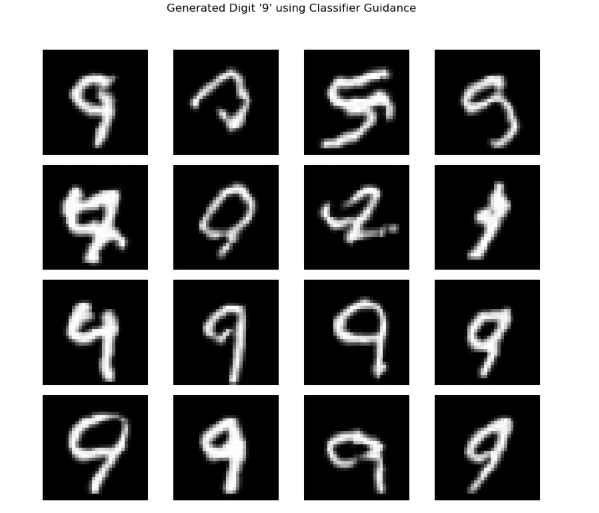
\includegraphics[width=0.65\linewidth]{images/guided_diffusion_results.png}
    \caption{Classifier-Guided Diffusion on MNIST: class `9' generations at guidance scale $\lambda=2.0$.}
    \label{fig:guided_diffusion_results}
\end{figure}

% =====================================================
\section{Dataset for Style-Transfer Evaluation}
\label{sec:dataset}

\noindent Before evaluating any existing style-aware diffusion systems, a focused dataset was curated to represent the kind of distribution shifts observed in the wild.
Approximately \textbf{500 images} were handpicked from publicly available sources such as Pinterest~\cite{pinterest}, iStock~\cite{istock}, and Google Images~\cite{google_images}, spanning a wide range of adverse environmental conditions such as fog, smog, heavy rain, snow, blizzard, sandstorm, dust storm, storm, and forest fire.
These scenes were specifically selected because both the background and foreground elements are often veiled under a strong stylistic ``shroud,'' which makes object boundaries ambiguous and significantly complicates classification and detection tasks.
This dataset serves as the common evaluation ground for all subsequent models.

\noindent \textbf{Note:} Although testing and benchmarking were carried out across all environmental domains mentioned above, the following visual comparisons and analyses focus specifically on the \textbf{agriculture domain}, which was found to most effectively resonate with the objectives of realistic distribution-shift representation and volumetric environmental stylisation.

\begin{figure}[!h]
    \centering
    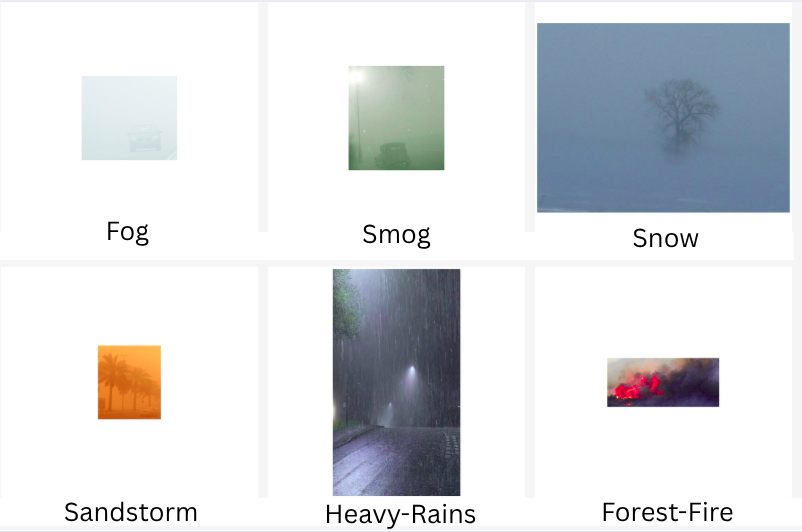
\includegraphics[width=\linewidth]{images/curated_dataset_collage.png}
    \caption{Representative collage from the curated dataset used for evaluation, spanning diverse environmental conditions such as fog, smog, snow, sandstorm, and forest fire. The agriculture domain subset (shown here) was selected for focused visual analysis due to its strong correspondence with real-world visibility and scattering effects.}
    \label{fig:curated_dataset_collage}
\end{figure}

% =====================================================
\section{Evaluation of Existing Style-Transfer Frameworks}
\label{sec:existing_solutions}

\noindent Three frameworks were evaluated in sequence, each representing a different philosophy for injecting style into a pretrained generative model.
The progression --- from auxiliary style network (StyleShot) to encoder-fusion (CSGO) to attention-block selection (InstantStyle) --- tells a story about where style actually lives in a diffusion model.

% -------------------------------------------------------
\subsection{StyleShot: One-Shot Style Transfer with Attention Modulation}
\label{sec:styleshot}

To explore prompt-guided, reference-based style transfer under environmental distribution shifts, the first existing solution evaluated was \textbf{StyleShot}~\cite{gao2024styleshot}.
These scenes were selected to intentionally represent the loss of visibility and structural ambiguity typical of style-induced distribution shifts, where both the background and foreground appear enveloped in a dense ``style shroud.''
The goal was to examine whether the model could convincingly reproduce such styles while maintaining semantic coherence.

\paragraph{Architecture Overview}
As illustrated in Figure~\ref{fig:styleshot_architecture}, the original StyleShot framework is designed as a \textbf{tri-modal diffusion system}, integrating three modalities --- text, content, and style --- into a unified diffusion backbone.
It consists of three encoders:
(1) a \textbf{Style-Aware Encoder} that partitions the style reference image into multiple scales and embeds each partition using transformer blocks (OpenCLIP ViT-H/14)~\cite{radford2021clip} to capture tone, colour, and texture statistics;
(2) a \textbf{Content-Fusion Encoder} that processes edge maps or structure references to maintain spatial layout; and
(3) a \textbf{CLIP Text Encoder} that provides semantic grounding for prompt-based control.
These embeddings are fused within the diffusion U-Net~\cite{ronneberger2015unet} via \textbf{Parallel Cross-Attention} and \textbf{Residual Addition}, enabling the network to modulate appearance (from the style image) while preserving textual and structural semantics.

\begin{figure}[!h]
    \centering
    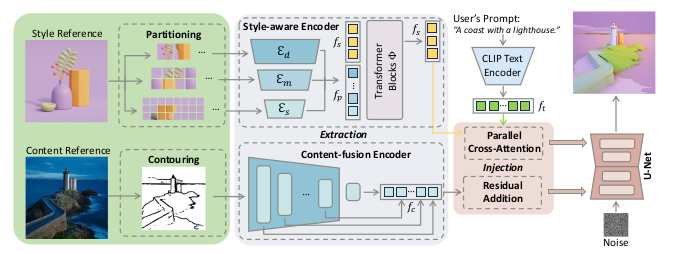
\includegraphics[width=0.75\linewidth]{images/styleshot_architecture.png}
    \caption{Overall architecture of StyleShot~\cite{gao2024styleshot}: tri-modal fusion of style, content, and text embeddings through parallel cross-attention and residual addition in the diffusion U-Net.}
    \label{fig:styleshot_architecture}
\end{figure}

\paragraph{Modified Experimental Configuration}
In this work, the setup was simplified to reflect the \textbf{text + style reference} configuration, as the curated dataset did not include explicit content reference images or edge maps.
Accordingly, the \textit{Content-Fusion Encoder} branch was disabled.
The model thus operated as a \textbf{bi-modal diffusion system}, driven by the CLIP text embeddings for semantic composition and the style-aware embeddings for texture and tone modulation.
The fusion occurred through parallel cross-attention layers within the diffusion U-Net, where style tokens ($f_s$) and text embeddings ($f_t$) jointly influenced the denoising trajectory:
\[
\text{Attn}_{\text{final}} = \text{Attn}(Q, K_t, V_t) + \lambda_s \, \text{Attn}(Q, K_s, V_s),
\]
with $\lambda_s$ controlling the relative style strength.

\paragraph{Results}
When evaluated on the curated dataset, StyleShot~\cite{gao2024styleshot} generated outputs that were visually rich but \textbf{overly artistic} and aesthetically biased rather than physically realistic.
The model often prioritised stylistic exaggeration over faithful reconstruction, producing textures reminiscent of oil painting or digital art.
This deficiency became evident in agricultural and outdoor scenes, where machinery and terrain edges remained sharply defined while the background appeared painterly and abstract.
Similarly, in underwater or snow-heavy conditions, StyleShot was unable to simulate realistic scattering, depth-based attenuation, or backscatter, producing flattened tones that lacked the characteristic absorption and haze structure seen in real imagery.

\begin{figure}[!h]
    \centering
    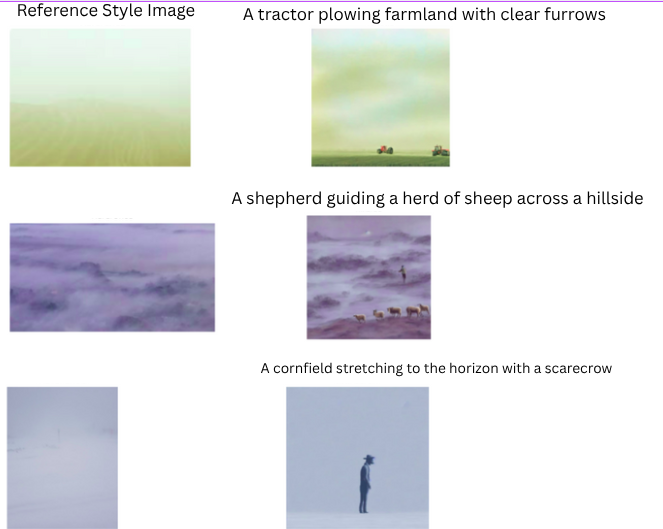
\includegraphics[width=0.85\linewidth]{images/styleshot_fail_agriculture.png}
    \caption{StyleShot on curated agricultural scenes: over-stylisation and lack of depth-consistent haze. Foreground regions remain overly sharp while the background becomes painterly.}
    \label{fig:styleshot_fail_agri}
\end{figure}

\paragraph{Inference}
StyleShot offers an elegant and training-free mechanism for reference-based style transfer but demonstrates clear limitations when applied to environmental domain adaptation tasks.
Its diffusion outputs are dominated by artistic stylisation, fail to produce realistic haze or scattering around the foreground, and often degrade structural fidelity.
These shortcomings motivate the exploration of more adaptive, physics-aware frameworks.

% -------------------------------------------------------
\subsection{CSGO: Content--Style Composition in Text-to-Image Generation}
\label{sec:csgo}

To assess an end-to-end trained alternative to tuning-free stylisation, \textbf{CSGO}~\cite{xing2024csgocomp} was evaluated on the curated extreme-conditions set.
The objective remains to transfer the environmental ``style shroud'' while preserving scene semantics and producing physically plausible depth-dependent effects.

\paragraph{Architecture Overview and Configuration}
CSGO is built on an SDXL backbone~\cite{podell2023sdxlimprovinglatentdiffusion} and explicitly \emph{decouples} content and style controls.
A \emph{content pathway} injects CLIP image encoder features~\cite{radford2021clip} via cross-attention in the down blocks and a \emph{Tile ControlNet} stream~\cite{zhang2023controlnet} in the up blocks.
In parallel, a \emph{style pathway} encodes the reference style image using a ViT-H encoder~\cite{dosovitskiy2020vit} and a Perceiver Resampler, injecting tokens into both the U-Net and ControlNet.
Training uses the IMAGStyle dataset (210k triplets) with content from MSRA10K/MSRA-B and styles from WikiArt and Midjourney.

\begin{figure}[!h]
    \centering
    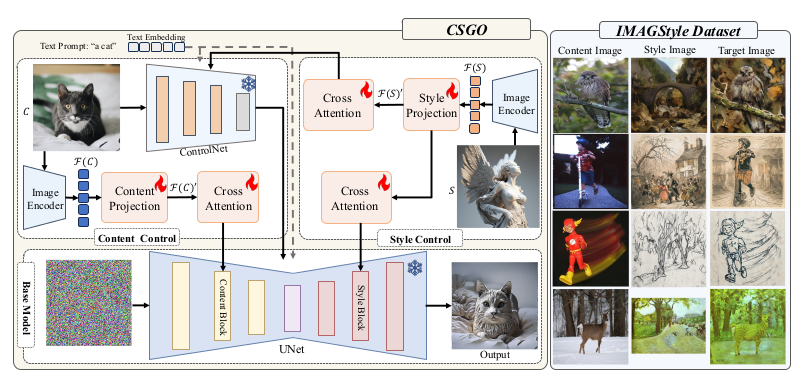
\includegraphics[width=0.75\linewidth]{images/csgo_architecture.png}
    \caption{Overview of the CSGO framework: decoupled content and style pathways fused into SDXL with ControlNet support (adapted from Xing et al., 2024~\cite{xing2024csgocomp}).}
    \label{fig:csgo_architecture}
\end{figure}

In this study, CSGO was run in a \textbf{text + style} regime (no content reference).
A blank canvas was provided as content input; prompts defined semantics, and the style image supplied appearance tokens.
ControlNet (Tile) was used at low conditioning scale (0.2).
Sampling used 50 steps, guidance 5.5, \texttt{style\_scale}=1.0, \texttt{content\_scale}=1.3.

\paragraph{Results}
CSGO delivered strong stylistic colour bias but lacked physics-consistent environmental haze.
Foregrounds stayed sharp while backgrounds were softly recoloured, failing to create volumetric occlusion.
Underwater and fog scenes lacked depth-dependent attenuation and scattering, producing flatter results.

\begin{figure}[!h]
    \centering
    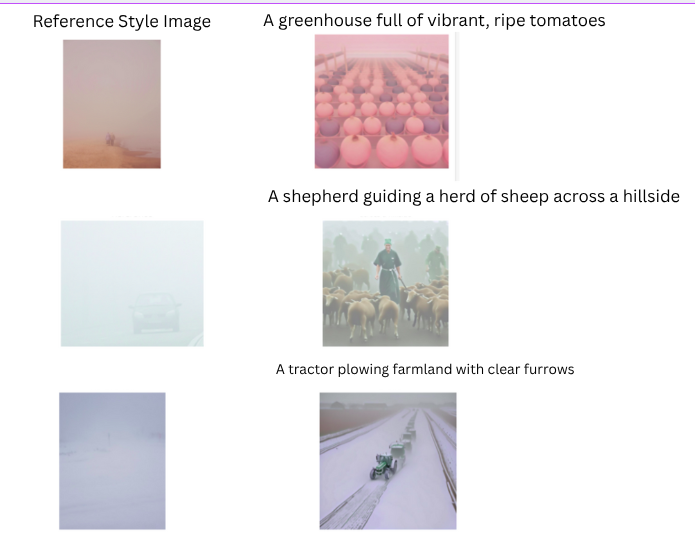
\includegraphics[width=0.85\linewidth]{images/csgo_fail_agriculture.png}
    \caption{CSGO on curated agricultural scenes (text+style setup): texture transfer without depth-consistent haze; crisp foreground edges.}
    \label{fig:csgo_fail_agri}
\end{figure}

\paragraph{Inference}
CSGO provides a solid framework for content--style separation but, in a text+style setup, lacks physical realism.
Without a content image prior or strong ControlNet, style behaves like recolouring rather than volumetric shrouding.
This motivates physics-aware guidance in later models.

% -------------------------------------------------------
\subsection{InstantStyle: Style-Preserving Injection with IP-Adapter}
\label{sec:instantstyle}

Among all evaluated methods, \textbf{InstantStyle}~\cite{wang2024instantstyle} consistently delivered physically grounded and semantically coherent text-guided style transfer across adverse environmental domains.
As a tuning-free adapter-based framework built on SDXL~\cite{podell2023sdxlimprovinglatentdiffusion}, it introduced a minimalist yet powerful mechanism for injecting style residuals directly into the diffusion process without modifying the base network weights.
This approach offered the best trade-off between \textit{semantic consistency, structural fidelity}, and \textit{visual realism}, setting the stage for adaptive variants such as InstantStyle-Plus~\cite{wang2024instantstyleplus}.

\paragraph{Architecture and Embedding Formulation}
InstantStyle augments the SDXL backbone with an additional Image Prompt Adapter (IP-Adapter~\cite{ye2023ipadapterfidelityadapters}) that encodes the style image in the same latent CLIP~\cite{radford2021clip} space as the text embedding.
Given a text prompt $t$ and a style image $I_s$, the system computes:
\[
\mathbf{e}_t = f_{\text{text}}(t), \qquad \mathbf{e}_s = f_{\text{img}}(I_s).
\]
To disentangle appearance from semantics, InstantStyle applies a subtraction in the CLIP feature space:
\[
\mathbf{e}_{\text{style}} = \mathbf{e}_s - \beta \, \mathbf{e}_t,
\]
where $\beta \in [0.6, 0.8]$ controls the degree of content suppression.
This residual embedding $\mathbf{e}_{\text{style}}$ encodes pure stylistic cues --- colour palette, illumination, texture statistics --- while discarding semantic overlap with the text description.
The resulting style tokens are linearly projected into the attention space of SDXL's U-Net via the IP-Adapter, forming key--value pairs $(\mathbf{K}_{\text{style}}, \mathbf{V}_{\text{style}}) = \mathcal{P}(\mathbf{e}_{\text{style}})$ that are injected into selected up-block cross-attention layers:
\[
\mathrm{Attn}_l(\mathbf{z}_l)
= \mathrm{softmax}\!\left(\frac{\mathbf{Q}_l \, [\mathbf{K}_t \, \| \, \mathbf{K}_{\text{style}}]^{\!\top}}{\sqrt{d}}\right)
[\mathbf{V}_t \, \| \, \mathbf{V}_{\text{style}}].
\]

\begin{figure}[!h]
    \centering
    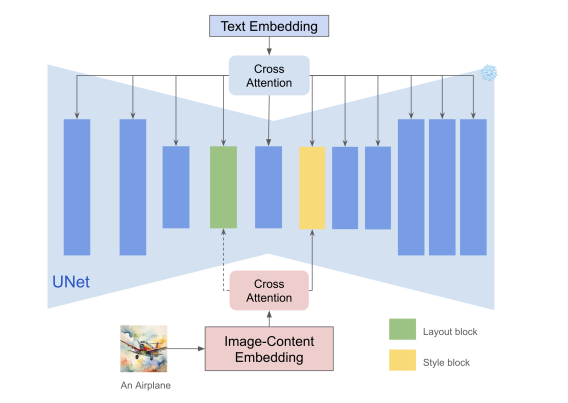
\includegraphics[width=0.7\linewidth]{images/instantstyle_architecture.png}
    \caption{InstantStyle architecture: CLIP-based text and style embeddings, residual subtraction, and IP-Adapter cross-attention injection into SDXL layers (adapted from Wang et al., 2024~\cite{wang2024instantstyle}).}
    \label{fig:instantstyle_architecture}
\end{figure}

\paragraph{Configuration and Modes}
Two principal modes were evaluated:
\begin{itemize}
    \item \textbf{Soft Mode:} 40 diffusion steps, guidance 6.8, and style scale 0.83 --- prioritising volumetric realism and semantic faithfulness.
    \item \textbf{Strong Mode:} Higher guidance and style scale, emphasising contrast and saturation at the expense of depth consistency.
\end{itemize}
Additionally, a \textbf{tuned-soft} variant relaxed anti-blur terms in the negative prompt (such as ``sharp focus'' and ``deformed'') to allow physically consistent diffusion of light and haze in weathered environments.

\paragraph{Results}
Across the agriculture domain, InstantStyle's tuned-soft configuration produced perceptually rich and physically consistent results.
The model achieved volumetric haze and subtle scattering effects while retaining the structural geometry of the base content.
Foreground objects remained coherent with the background illumination, demonstrating the framework's ability to generalise to unseen distributions without explicit retraining.

\begin{figure}[!h]
    \centering
    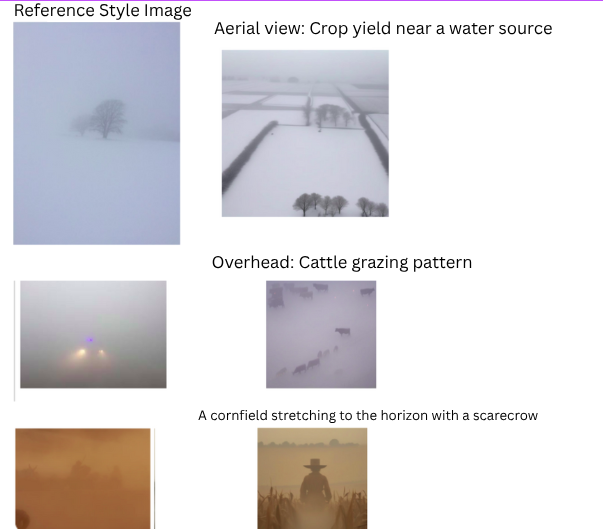
\includegraphics[width=0.65\linewidth]{images/instantstyle_results.png}
    \caption{InstantStyle results on the agriculture benchmark: the tuned-soft variant maintains volumetric realism and illumination consistency; strong mode exaggerates stylisation.}
    \label{fig:instantstyle_results}
\end{figure}

\paragraph{Summary}
InstantStyle thus serves as the \textbf{foundational bridge} between appearance injection and semantic conditioning under environmental distribution shift.
While StyleShot offered aesthetic coherence and CSGO achieved explicit disentanglement, only InstantStyle reached a consistent equilibrium between physical plausibility and semantic precision.
This balance motivated its natural evolution into \textbf{InstantStyle-Plus}~\cite{wang2024instantstyleplus}, where ControlNet~\cite{zhang2023controlnet} spatial priors and CSD~\cite{somepalli2024csd}-guided perceptual constraints extend the architecture toward adaptive, context-aware diffusion.

\begin{table}[!h]
\centering
\caption{Qualitative comparison of existing style-transfer frameworks on extreme-atmospheric content.}
\label{tab:existing_solutions_comparison}
\renewcommand{\arraystretch}{1.3}
\begin{tabularx}{\textwidth}{lXXX}
\toprule
\textbf{Method} & \textbf{Semantic Fidelity} & \textbf{Atmospheric Realism} & \textbf{Key Limitation} \\
\midrule
StyleShot & High & Low & Transfers global mood, not physical texture; over-artistic \\
CSGO & Medium--High & Low--Medium & Layout leakage; flat recolouring without volumetric depth \\
InstantStyle (all-block) & Low & Medium & Style reference geometry overrides content structure \\
InstantStyle (block-selective) & High & Medium & Style is perceptual, not physically grounded \\
\bottomrule
\end{tabularx}
\end{table}

% -------------------------------------------------------
\FloatBarrier
\subsection{Summary}
\label{sec:comparison_existing}

\noindent The foundational experiments --- Vision Transformer, U-Net, DDPM, and classifier-guided diffusion --- provided a cohesive understanding of the mechanisms behind diffusion-based image generation, grounding the theory and establishing the building blocks for the style-aware frameworks evaluated in the second half of this chapter.
The pattern across StyleShot, CSGO, and InstantStyle is clear: the best performers at semantic fidelity produced the least atmospheric realism, and vice versa.
None of the three frameworks had any mechanism to make style injection \emph{physically consistent with scene depth} --- a sandstorm should attenuate objects in proportion to their distance from the camera, but all three systems apply the style shift uniformly across the image.
Bridging this gap was the motivation for the methods developed in subsequent chapters.
The proposed style transfer method --- V0 (InstantStyle with CSD Guidance, Chapter~\ref{chap:adaptive_proposed}) --- reduces CLIP ViT-L-14 confidence from 0.620--0.698 for these passive baselines down to 0.514; the physics pipeline V3 (Chapter~\ref{chap:phase2_pipeline}), by replacing global style injection with depth-consistent Koschmieder compositing, reduces it further to \textbf{0.274} --- a 56\,\% reduction relative to the best passive baseline and 47\,\% below V0.
